\begin{frame}[parent={ie:agenda}, hasnext=true, hasprev=false]
\frametitle{Definição de processo}

\begin{block:fact}{Aplicações}
	\begin{itemize}
		\item Por definição, representa precisamente um processo (e as inconsistências
		porventura existentes)
		
		\item Simulação
		\begin{itemize}
			\item SimSE:  \url{https://www.youtube.com/watch?v=lJpHPJrj6Pc}
			\item Simulação baseada em eventos discretos
			\item Simulação baseada em agentes
		\end{itemize}
		
		\item Treinamento
		
		\item Criação de ambientes centrados em processos (PSEE)
	\end{itemize}
\end{block:fact}
\end{frame}

\begin{frame}[hasnext=true, hasprev=true]
	\frametitle{Definição de processo}

	
	\begin{block:concept}{Linguagem para modelagem de processos}
		Linguagens de modelagem de processo permitem a representação de atividades,
		papéis, artefatos e ferramentas necessários a um processo.
	\end{block:concept}
	
	\begin{block:fact}{Exemplos}
		\begin{itemize}
			\item Redes de Petri
			\item BPML
			\item SPEM
			\item Linguagens de programação de uso geral (``Software processes are software too'')
		\end{itemize}
	\end{block:fact}
\end{frame}


\begin{frame}
	\frametitle{Definição de processo}
	\framesubtitle{Redes de Petri}
	
	\begin{block:concept}{Rede de Petri}
		Modelo formal para descrição de sistemas de eventos discretos.
	\end{block:concept}
	
	\begin{block:concept}{Estrutura}
		\begin{itemize}
			\item Lugares (passivo, representa condições, recursos, etc)
			\item Transições (ativo, representa eventos ou ações)
			\item Arcos (relação entre transição e lugar)
		\end{itemize}
	\end{block:concept}

	\begin{block:concept}{Token e marcação}
	\begin{itemize}
		\item Token: item de informação (sempre associado a um lugar).
		\item Marcação: associação de tokens com os lugares na rede.
	\end{itemize}
	\end{block:concept}
\end{frame}

\begin{frame}
	\frametitle{Definição de processo}
	\framesubtitle{Redes de Petri}
	
	\begin{block:concept}{Rede de Petri}
		Modelo formal para descrição de sistemas de eventos discretos.
	\end{block:concept}
	
	\begin{block:concept}{Funcionamento}
	\begin{itemize}
		\item Execução de uma rede de Petri é controlada pela marcação da rede
		\begin{itemize}
			\item Marcação muda com a execução da rede
		\end{itemize}
		
		\item Cada ficha controla a execução das transições
		\begin{itemize}
			\item Transição é habilitada se existe, para cada um de seus lugares de
			entrada, uma quantidade de fichas igual ou maior à multiplicidade daquele
			lugar em relação à transição.
			
			\item Uma vez habilitada, uma transição pode ser disparada
			\begin{itemize}
				\item Retiram-se fichas do lugar de entrada (uma ficha para cada
				associação lugar/transição),
				\item Colocam-se fichas nos lugares de saída (uma ficha para cada
				associação transição/lugar).
			\end{itemize}
		\end{itemize}
	\end{itemize}
\end{block:concept}
\end{frame}

\begin{frame}
	\frametitle{Rede de Petri}
	\framesubtitle{Funcionamento}
	
	\begin{block:ie}{Exemplos}
		\centering
		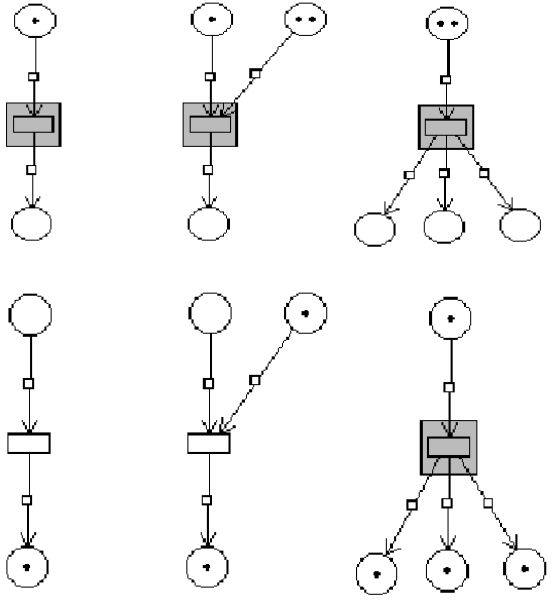
\includegraphics[width=.5\textwidth]{software-engineering/petri-net/petrinet-execution-examples-v2}
	\end{block:ie}
\end{frame}


\begin{frame}
	\frametitle{Rede de Petri}
	\framesubtitle{Funcionamento}
	
	\begin{block:ie}{Mais um exemplo (1/2)}
		\centering
		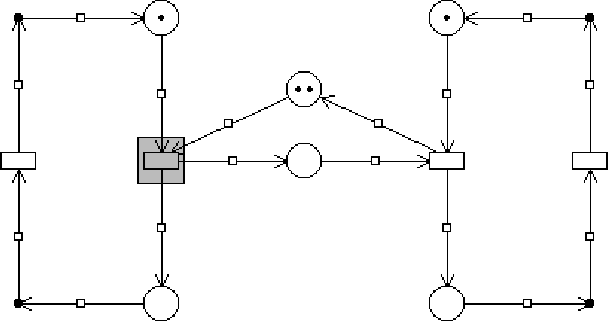
\includegraphics[width=.85\textwidth]{software-engineering/petri-net/petrinet-execution-example1-1}
	\end{block:ie}
\end{frame}

\begin{frame}
	\frametitle{Rede de Petri}
	\framesubtitle{Funcionamento}
	
	\begin{block:ie}{Mais um exemplo (2/2)}
		\centering
		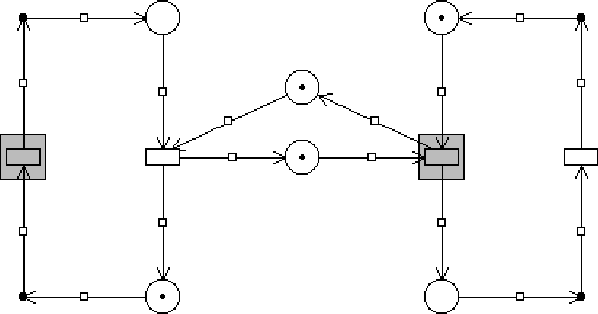
\includegraphics[width=.85\textwidth]{software-engineering/petri-net/petrinet-execution-example1-2}
	\end{block:ie}
\end{frame}


\begin{frame}
	\frametitle{Rede de Petri colorida}
	
	\begin{block:ie}{Exemplo}
		\centering
		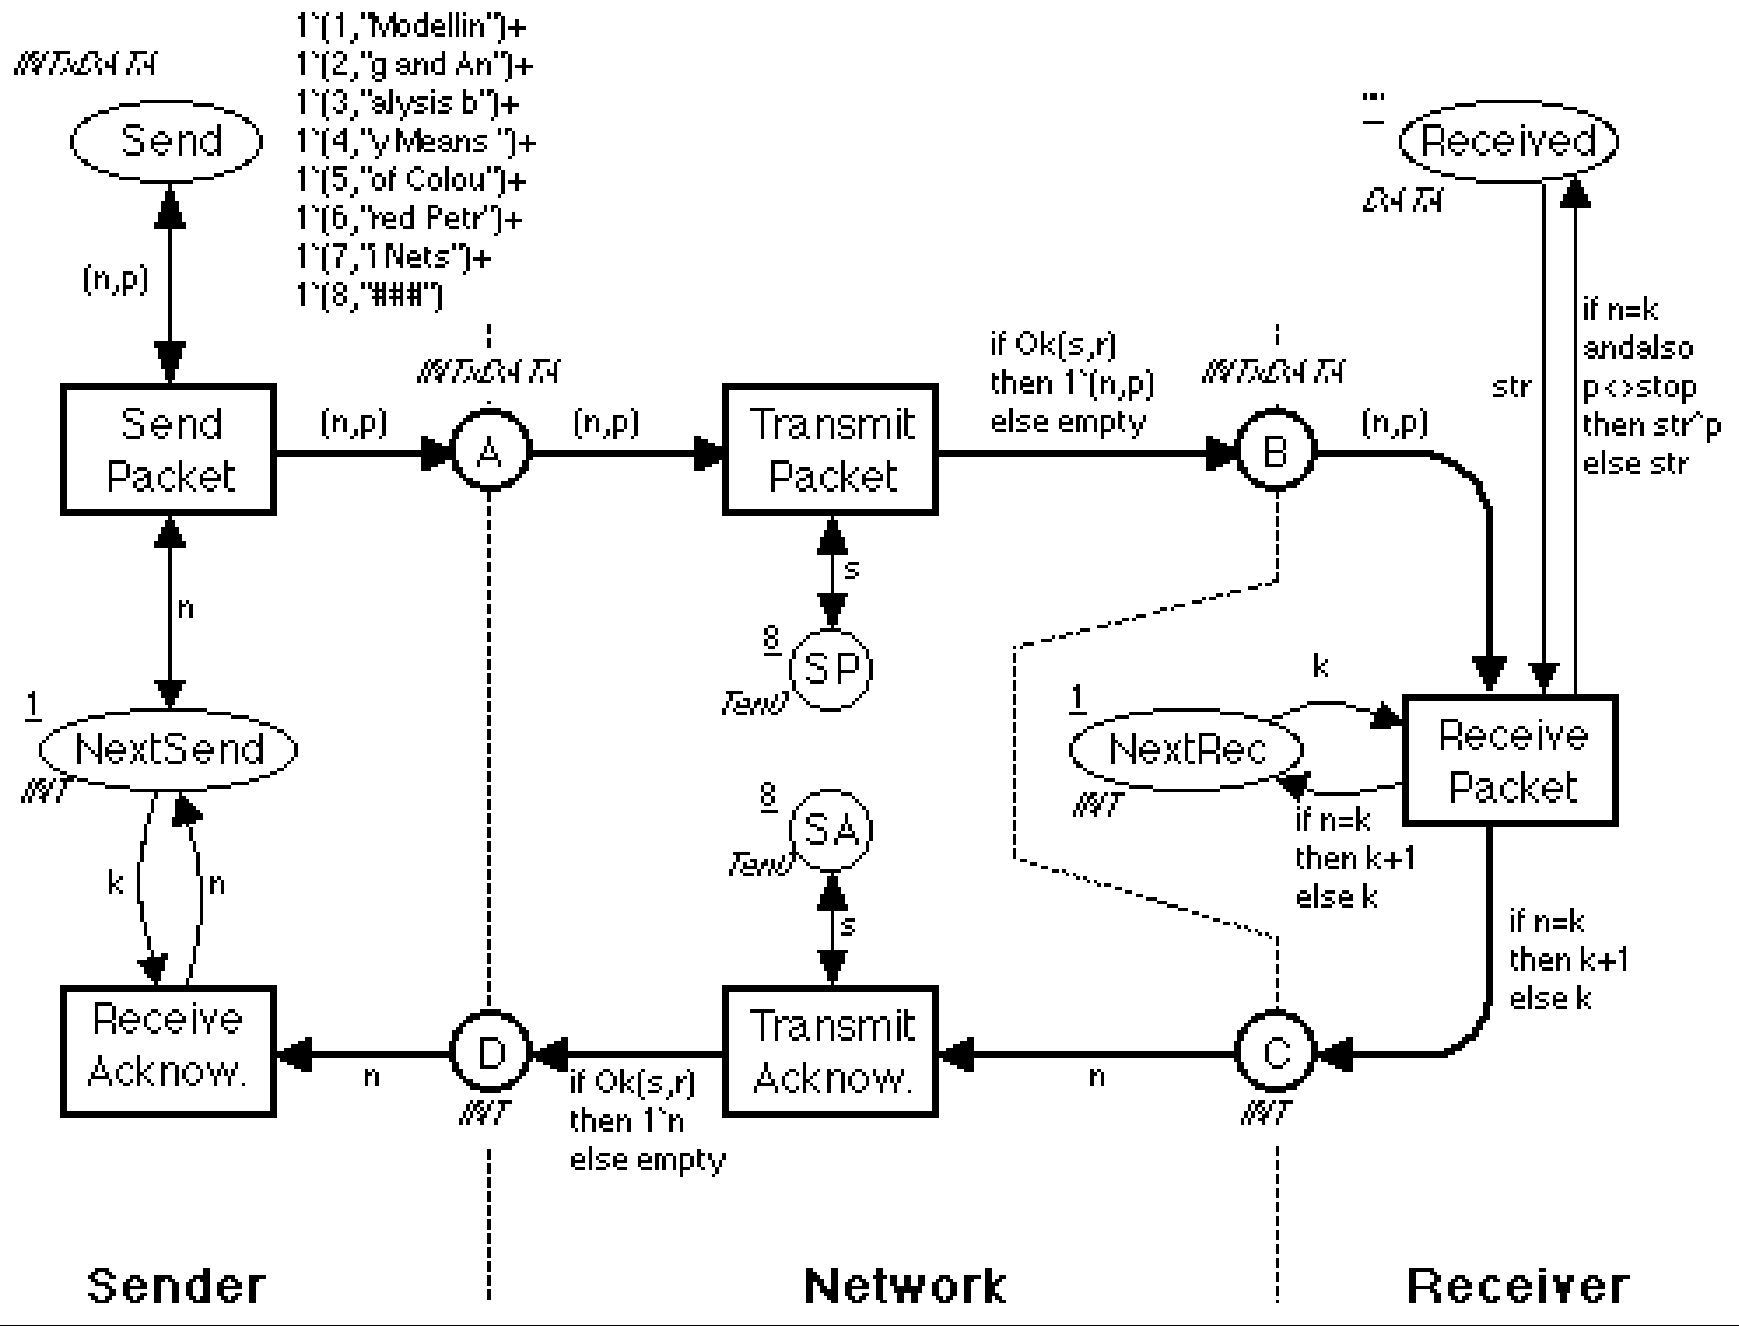
\includegraphics[width=.85\textwidth]{software-engineering/petri-net/cpn-example-network_protocol}
	\end{block:ie}
\end{frame}



\begin{frame}
	\frametitle{Definição de processo}
	\framesubtitle{BPML}
	
	
	
	\begin{block:fact}{Exemplos}
		\begin{itemize}
			\item SEI (Base de conhecimento)
			
			\item \url{https://josegomezdev.medium.com/full-software-development-life-cycle-ca80bb6aae21}
		\end{itemize}
	\end{block:fact}
\end{frame}


\begin{frame}
	\frametitle{Definição de processo}
	\framesubtitle{SPEM}
	
	
	
	\begin{block:fact}{Scrum}
		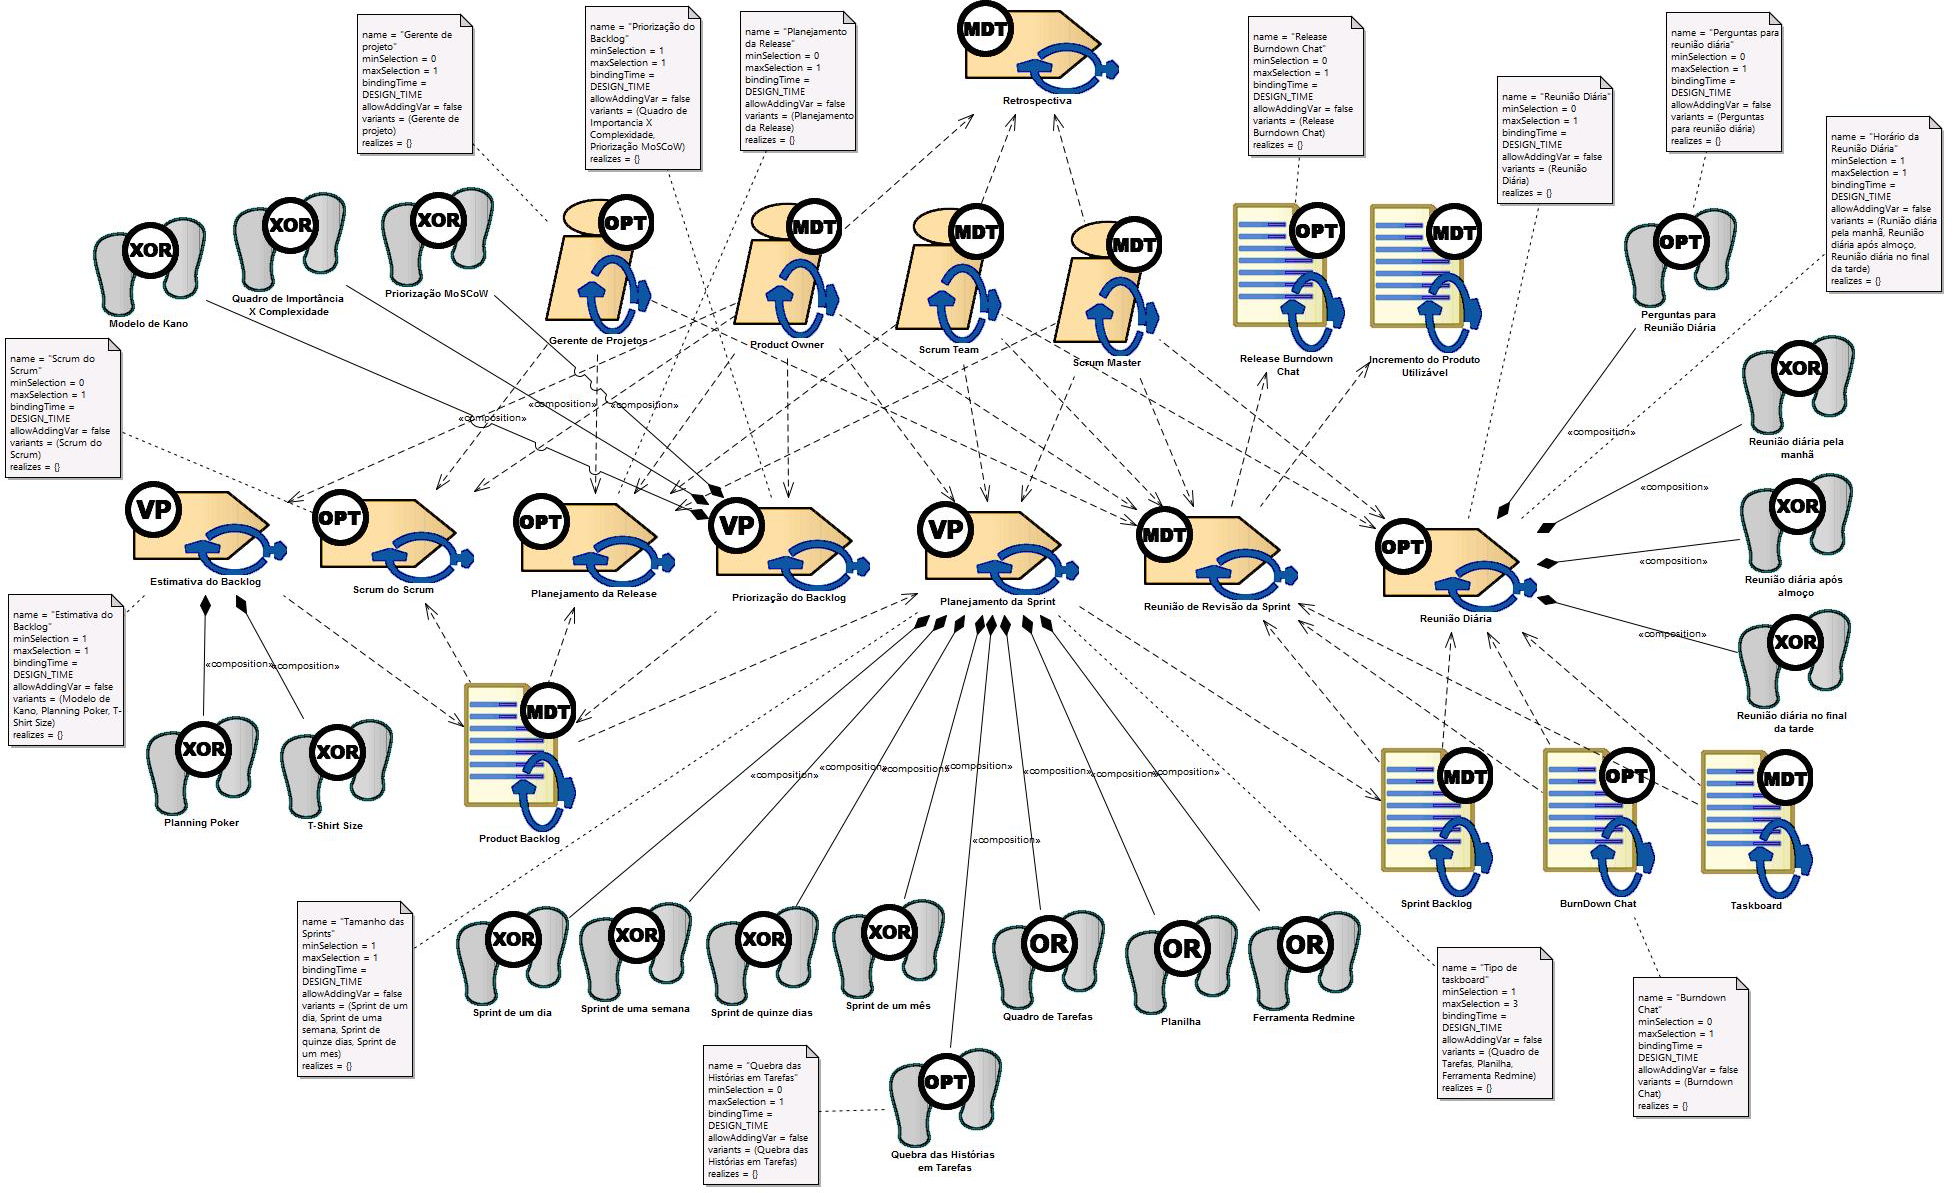
\includegraphics[width=\textwidth]{scrumsprl}
	\end{block:fact}
\end{frame}



\begin{frame}
	\frametitle{Definição de processo}
	\framesubtitle{EPF}
	
	
	\begin{block:concept}{Definição}
		Abordagem composicional que permite a edição, configuração e publicação de processos
		de software.
	\end{block:concept}
	
	\begin{block:fact}{Componentes}
		\begin{itemize}
			\item Method Content: padroniza a representação e gerencia bibliotecas de componentes
			reutilizáveis. Possui a definição de papeis, tarefas, produtos de trabalho e seus
			relacionamentos;
			
			\item Process: determina a sequência das fases, iterações e atividades, e define
			quando realizar as tarefas;
			
			\item Plug-ins: representam um conjunto de Method Content e Process, permitindo a
			customização de um processo;
			
			\item Configurations: seleção de um subconjunto de Method Content para ser
			publicado, visando atender as necessidades de um determinado projeto.
		\end{itemize}
	\end{block:fact}
\end{frame}


\begin{frame}
	\frametitle{Definição de processo}
	\framesubtitle{EPF}
	
	\begin{block:fact}{Exemplos}
		\begin{itemize}
			\item OpenUP: \url{https://magsilva.pro.br/teaching/epf-processes/OpenUP/index.htm}
			\item XP: \url{https://magsilva.pro.br/teaching/epf-processes/XP/index.htm}
			\item Scrum: \url{https://magsilva.pro.br/teaching/epf-processes/Scrum/index.htm}
		\end{itemize}
	\end{block:fact}
\end{frame}


\begin{frame}
	\frametitle{Definição de processo}
	\framesubtitle{EPF}
	
	\begin{block:concept}{Mecanismos para evolução do processo}
		O EPF permite representar variabilidade de artefatos para o controle da evolução e reuso de processos:

		\begin{itemize}
			\item Contribui - adiciona um novo elemento ao elemento base;

			\item Substitui - substitui o elemento base por um novo elemento;

			\item Estende - estende um elemento com as características de um elemento base;

			\item Estende e Substitui - substitui somente os atributos que foram modificados em um novo elemento.
		\end{itemize}
	\end{block:concept}
\end{frame}

%\begin{frame}
%	\frametitle{Definição de processo}
%	\framesubtitle{Linhas de processo de software}
%	
%	\begin{block:concept}{Definição}
%		Estabelece técnicas e mecanismos para a modelagem de similaridades e variabilidades
%		existentes em uma família de processos de software, e a derivação de processos de
%		software customizados que atendam às necessidades específicas de um determinado
%		projeto de desenvolvimento de software.
%	\end{block:concept}
%\end{frame}
%
%
%\begin{frame}[hasnext=false, hasprev=true]
%	\frametitle{Definição de processo}
%	\framesubtitle{Linhas de processo de software}
%	
%	\begin{block:fact}{Exemplo: Scrum}
%		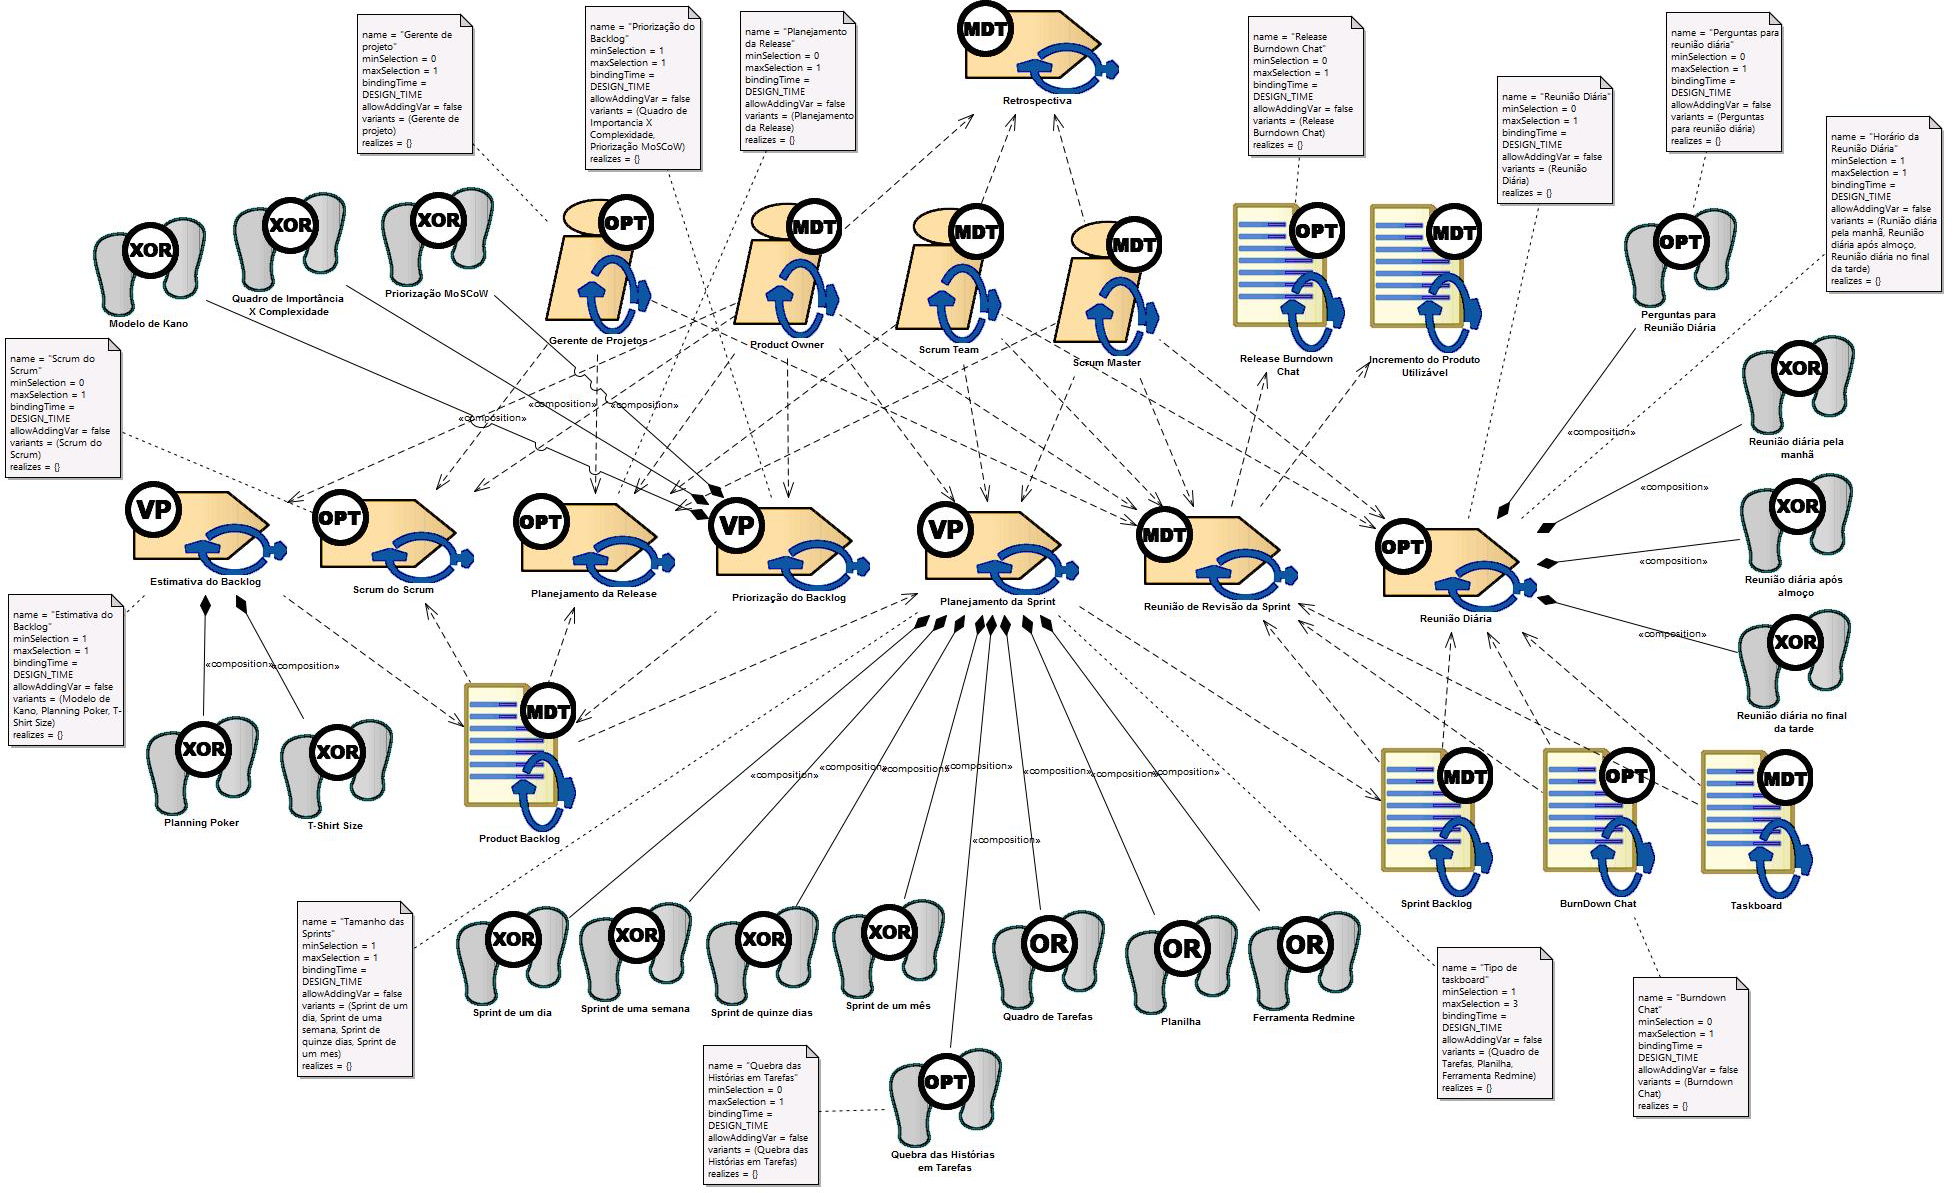
\includegraphics[width=\textwidth]{scrumsprl}
%	\end{block:fact}
%	
%	\note{Linha de Produto para o Scrum, definida com a abordagem composicional SMartySPEM pelo
%	Jaime Dias e Edson Oliveira Jr., da UEM.}
%\end{frame}


